\PassOptionsToPackage{unicode=true}{hyperref} % options for packages loaded elsewhere
\PassOptionsToPackage{hyphens}{url}
%
\documentclass[]{article}
\usepackage{lmodern}
\usepackage{amssymb,amsmath}
\usepackage{ifxetex,ifluatex}
\usepackage{fixltx2e} % provides \textsubscript
\ifnum 0\ifxetex 1\fi\ifluatex 1\fi=0 % if pdftex
  \usepackage[T1]{fontenc}
  \usepackage[utf8]{inputenc}
  \usepackage{textcomp} % provides euro and other symbols
\else % if luatex or xelatex
  \usepackage{unicode-math}
  \defaultfontfeatures{Ligatures=TeX,Scale=MatchLowercase}
\fi
% use upquote if available, for straight quotes in verbatim environments
\IfFileExists{upquote.sty}{\usepackage{upquote}}{}
% use microtype if available
\IfFileExists{microtype.sty}{%
\usepackage[]{microtype}
\UseMicrotypeSet[protrusion]{basicmath} % disable protrusion for tt fonts
}{}
\IfFileExists{parskip.sty}{%
\usepackage{parskip}
}{% else
\setlength{\parindent}{0pt}
\setlength{\parskip}{6pt plus 2pt minus 1pt}
}
\usepackage{hyperref}
\hypersetup{
            pdftitle={Project 1},
            pdfauthor={Christy Cao},
            pdfborder={0 0 0},
            breaklinks=true}
\urlstyle{same}  % don't use monospace font for urls
\usepackage[margin=1in]{geometry}
\usepackage{color}
\usepackage{fancyvrb}
\newcommand{\VerbBar}{|}
\newcommand{\VERB}{\Verb[commandchars=\\\{\}]}
\DefineVerbatimEnvironment{Highlighting}{Verbatim}{commandchars=\\\{\}}
% Add ',fontsize=\small' for more characters per line
\usepackage{framed}
\definecolor{shadecolor}{RGB}{248,248,248}
\newenvironment{Shaded}{\begin{snugshade}}{\end{snugshade}}
\newcommand{\AlertTok}[1]{\textcolor[rgb]{0.94,0.16,0.16}{#1}}
\newcommand{\AnnotationTok}[1]{\textcolor[rgb]{0.56,0.35,0.01}{\textbf{\textit{#1}}}}
\newcommand{\AttributeTok}[1]{\textcolor[rgb]{0.77,0.63,0.00}{#1}}
\newcommand{\BaseNTok}[1]{\textcolor[rgb]{0.00,0.00,0.81}{#1}}
\newcommand{\BuiltInTok}[1]{#1}
\newcommand{\CharTok}[1]{\textcolor[rgb]{0.31,0.60,0.02}{#1}}
\newcommand{\CommentTok}[1]{\textcolor[rgb]{0.56,0.35,0.01}{\textit{#1}}}
\newcommand{\CommentVarTok}[1]{\textcolor[rgb]{0.56,0.35,0.01}{\textbf{\textit{#1}}}}
\newcommand{\ConstantTok}[1]{\textcolor[rgb]{0.00,0.00,0.00}{#1}}
\newcommand{\ControlFlowTok}[1]{\textcolor[rgb]{0.13,0.29,0.53}{\textbf{#1}}}
\newcommand{\DataTypeTok}[1]{\textcolor[rgb]{0.13,0.29,0.53}{#1}}
\newcommand{\DecValTok}[1]{\textcolor[rgb]{0.00,0.00,0.81}{#1}}
\newcommand{\DocumentationTok}[1]{\textcolor[rgb]{0.56,0.35,0.01}{\textbf{\textit{#1}}}}
\newcommand{\ErrorTok}[1]{\textcolor[rgb]{0.64,0.00,0.00}{\textbf{#1}}}
\newcommand{\ExtensionTok}[1]{#1}
\newcommand{\FloatTok}[1]{\textcolor[rgb]{0.00,0.00,0.81}{#1}}
\newcommand{\FunctionTok}[1]{\textcolor[rgb]{0.00,0.00,0.00}{#1}}
\newcommand{\ImportTok}[1]{#1}
\newcommand{\InformationTok}[1]{\textcolor[rgb]{0.56,0.35,0.01}{\textbf{\textit{#1}}}}
\newcommand{\KeywordTok}[1]{\textcolor[rgb]{0.13,0.29,0.53}{\textbf{#1}}}
\newcommand{\NormalTok}[1]{#1}
\newcommand{\OperatorTok}[1]{\textcolor[rgb]{0.81,0.36,0.00}{\textbf{#1}}}
\newcommand{\OtherTok}[1]{\textcolor[rgb]{0.56,0.35,0.01}{#1}}
\newcommand{\PreprocessorTok}[1]{\textcolor[rgb]{0.56,0.35,0.01}{\textit{#1}}}
\newcommand{\RegionMarkerTok}[1]{#1}
\newcommand{\SpecialCharTok}[1]{\textcolor[rgb]{0.00,0.00,0.00}{#1}}
\newcommand{\SpecialStringTok}[1]{\textcolor[rgb]{0.31,0.60,0.02}{#1}}
\newcommand{\StringTok}[1]{\textcolor[rgb]{0.31,0.60,0.02}{#1}}
\newcommand{\VariableTok}[1]{\textcolor[rgb]{0.00,0.00,0.00}{#1}}
\newcommand{\VerbatimStringTok}[1]{\textcolor[rgb]{0.31,0.60,0.02}{#1}}
\newcommand{\WarningTok}[1]{\textcolor[rgb]{0.56,0.35,0.01}{\textbf{\textit{#1}}}}
\usepackage{graphicx,grffile}
\makeatletter
\def\maxwidth{\ifdim\Gin@nat@width>\linewidth\linewidth\else\Gin@nat@width\fi}
\def\maxheight{\ifdim\Gin@nat@height>\textheight\textheight\else\Gin@nat@height\fi}
\makeatother
% Scale images if necessary, so that they will not overflow the page
% margins by default, and it is still possible to overwrite the defaults
% using explicit options in \includegraphics[width, height, ...]{}
\setkeys{Gin}{width=\maxwidth,height=\maxheight,keepaspectratio}
\setlength{\emergencystretch}{3em}  % prevent overfull lines
\providecommand{\tightlist}{%
  \setlength{\itemsep}{0pt}\setlength{\parskip}{0pt}}
\setcounter{secnumdepth}{0}
% Redefines (sub)paragraphs to behave more like sections
\ifx\paragraph\undefined\else
\let\oldparagraph\paragraph
\renewcommand{\paragraph}[1]{\oldparagraph{#1}\mbox{}}
\fi
\ifx\subparagraph\undefined\else
\let\oldsubparagraph\subparagraph
\renewcommand{\subparagraph}[1]{\oldsubparagraph{#1}\mbox{}}
\fi

% set default figure placement to htbp
\makeatletter
\def\fps@figure{htbp}
\makeatother


\title{Project 1}
\author{Christy Cao}
\date{3/15/2020}

\begin{document}
\maketitle

\textbf{Introduction}

For this project, I will be analyzing the number of arrests for violent
crimes and poverty percentage of each of the US states. Because laws and
regulations can have a large impact on the safety and status of living
of a state, I decided to include the major political party of each
state. The examination of these variables can depict any differences/
correlations between Republican vs Democrat states in relation to the
violent crimes and poverty percentages. With this information, we can
generalize the protection from crime each state provides, and the
general quality of living of each state through it's crime rates and
poverty percentages. We can go on to find out which state is potentially
the safest/ most dangerous to live in and have a general idea of the
representation of each state. I found all datasets online/ Google.

\begin{Shaded}
\begin{Highlighting}[]
\CommentTok{#Data sets}
\CommentTok{#Data set #1: Violent Crime Rates by US State}
\KeywordTok{library}\NormalTok{(readr)}
\NormalTok{crime <-}\StringTok{ }\KeywordTok{read_csv}\NormalTok{(}\StringTok{"USArrests.csv"}\NormalTok{)}
\end{Highlighting}
\end{Shaded}

\begin{verbatim}
## Parsed with column specification:
## cols(
##   State = col_character(),
##   Murder = col_double(),
##   Assault = col_double(),
##   UrbanPop = col_double(),
##   Rape = col_double()
## )
\end{verbatim}

\begin{Shaded}
\begin{Highlighting}[]
\KeywordTok{head}\NormalTok{(crime)}
\end{Highlighting}
\end{Shaded}

\begin{verbatim}
## # A tibble: 6 x 5
##   State      Murder Assault UrbanPop  Rape
##   <chr>       <dbl>   <dbl>    <dbl> <dbl>
## 1 Alabama      13.2     236       58  21.2
## 2 Alaska       10       263       48  44.5
## 3 Arizona       8.1     294       80  31  
## 4 Arkansas      8.8     190       50  19.5
## 5 California    9       276       91  40.6
## 6 Colorado      7.9     204       78  38.7
\end{verbatim}

\begin{Shaded}
\begin{Highlighting}[]
\CommentTok{#Data set #2: Road Accident Deaths in US States}
\NormalTok{pov <-}\StringTok{ }\KeywordTok{read_csv}\NormalTok{(}\StringTok{"est18ustheOne.csv"}\NormalTok{, }
    \DataTypeTok{skip =} \DecValTok{1}\NormalTok{)}
\end{Highlighting}
\end{Shaded}

\begin{verbatim}
## Warning: Missing column names filled in: 'X5' [5], 'X6' [6], 'X7' [7],
## 'X8' [8], 'X9' [9], 'X10' [10], 'X11' [11], 'X12' [12], 'X13' [13], 'X14' [14],
## 'X15' [15], 'X16' [16], 'X17' [17], 'X18' [18], 'X19' [19], 'X20' [20],
## 'X21' [21], 'X22' [22], 'X23' [23], 'X24' [24], 'X25' [25]
\end{verbatim}

\begin{verbatim}
## Parsed with column specification:
## cols(
##   .default = col_logical(),
##   Name = col_character(),
##   `Poverty Percent, All Ages` = col_double(),
##   `90% CI Lower Bound` = col_double(),
##   `90% CI Upper Bound` = col_double()
## )
\end{verbatim}

\begin{verbatim}
## See spec(...) for full column specifications.
\end{verbatim}

\begin{Shaded}
\begin{Highlighting}[]
\KeywordTok{head}\NormalTok{(pov)}
\end{Highlighting}
\end{Shaded}

\begin{verbatim}
## # A tibble: 6 x 25
##   Name  `Poverty Percen~ `90% CI Lower B~ `90% CI Upper B~ X5    X6    X7   
##   <chr>            <dbl>            <dbl>            <dbl> <lgl> <lgl> <lgl>
## 1 Alab~             16.8             16.5             17.1 NA    NA    NA   
## 2 Alas~             11.1             10.5             11.7 NA    NA    NA   
## 3 Ariz~             14.1             13.8             14.4 NA    NA    NA   
## 4 Arka~             16.8             16.3             17.3 NA    NA    NA   
## 5 Cali~             12.8             12.7             12.9 NA    NA    NA   
## 6 Colo~              9.7              9.5              9.9 NA    NA    NA   
## # ... with 18 more variables: X8 <lgl>, X9 <lgl>, X10 <lgl>, X11 <lgl>,
## #   X12 <lgl>, X13 <lgl>, X14 <lgl>, X15 <lgl>, X16 <lgl>, X17 <lgl>,
## #   X18 <lgl>, X19 <lgl>, X20 <lgl>, X21 <lgl>, X22 <lgl>, X23 <lgl>,
## #   X24 <lgl>, X25 <lgl>
\end{verbatim}

\begin{Shaded}
\begin{Highlighting}[]
\CommentTok{#Data set #3: Political party of each state }
\KeywordTok{library}\NormalTok{(readr)}
\NormalTok{pol <-}\StringTok{ }\KeywordTok{read_csv}\NormalTok{(}\StringTok{"stateparty.csv"}\NormalTok{, }
    \DataTypeTok{col_types =} \KeywordTok{cols}\NormalTok{(}\StringTok{`}\DataTypeTok{Political Party}\StringTok{`}\NormalTok{ =}\StringTok{ }\KeywordTok{col_character}\NormalTok{(), }
        \DataTypeTok{State =} \KeywordTok{col_character}\NormalTok{()))}
\KeywordTok{head}\NormalTok{(pol)}
\end{Highlighting}
\end{Shaded}

\begin{verbatim}
## # A tibble: 6 x 2
##   State      `Political Party`
##   <chr>      <chr>            
## 1 Alabama    Republican       
## 2 Alaska     Republican       
## 3 Arizona    Republican       
## 4 Arkansas   Republican       
## 5 California Democrat         
## 6 Colorado   Democrat
\end{verbatim}

\textbf{Tidying / Joining }

To begin working with the datasets I was interested in, I had to combine
the 3 different datasets into one. After doing so, I was able to untidy/
tidy the dataset to show my understanding.

\begin{Shaded}
\begin{Highlighting}[]
\CommentTok{#Tidying / Joining}
\KeywordTok{library}\NormalTok{(dplyr)}
\end{Highlighting}
\end{Shaded}

\begin{verbatim}
## 
## Attaching package: 'dplyr'
\end{verbatim}

\begin{verbatim}
## The following objects are masked from 'package:stats':
## 
##     filter, lag
\end{verbatim}

\begin{verbatim}
## The following objects are masked from 'package:base':
## 
##     intersect, setdiff, setequal, union
\end{verbatim}

\begin{Shaded}
\begin{Highlighting}[]
\KeywordTok{library}\NormalTok{(tidyverse)}
\end{Highlighting}
\end{Shaded}

\begin{verbatim}
## -- Attaching packages ---------------------------------------------------------- tidyverse 1.3.0 --
\end{verbatim}

\begin{verbatim}
## v ggplot2 3.3.0     v purrr   0.3.4
## v tibble  3.0.1     v stringr 1.4.0
## v tidyr   1.0.3     v forcats 0.5.0
\end{verbatim}

\begin{verbatim}
## -- Conflicts ------------------------------------------------------------- tidyverse_conflicts() --
## x dplyr::filter() masks stats::filter()
## x dplyr::lag()    masks stats::lag()
\end{verbatim}

\begin{Shaded}
\begin{Highlighting}[]
\NormalTok{crime<-crime}\OperatorTok\KeywordTok{select}\NormalTok{(}\OperatorTok{-}\NormalTok{UrbanPop)}
\NormalTok{pov<-pov}\OperatorTok\KeywordTok{select}\NormalTok{(}\StringTok{"Name"}\NormalTok{, }\StringTok{"Poverty Percent, All Ages"}\NormalTok{)}
\NormalTok{merged1<-}\KeywordTok{full_join}\NormalTok{(crime,pov, }\DataTypeTok{by=}\KeywordTok{c}\NormalTok{(}\StringTok{"State"}\NormalTok{=}\StringTok{"Name"}\NormalTok{))}
\KeywordTok{glimpse}\NormalTok{(merged1)}
\end{Highlighting}
\end{Shaded}

\begin{verbatim}
## Rows: 50
## Columns: 5
## $ State                       <chr> "Alabama", "Alaska", "Arizona", "Arkans...
## $ Murder                      <dbl> 13.2, 10.0, 8.1, 8.8, 9.0, 7.9, 3.3, 5....
## $ Assault                     <dbl> 236, 263, 294, 190, 276, 204, 110, 238,...
## $ Rape                        <dbl> 21.2, 44.5, 31.0, 19.5, 40.6, 38.7, 11....
## $ `Poverty Percent, All Ages` <dbl> 16.8, 11.1, 14.1, 16.8, 12.8, 9.7, 10.3...
\end{verbatim}

\begin{Shaded}
\begin{Highlighting}[]
\NormalTok{merged<-}\KeywordTok{full_join}\NormalTok{(merged1, pol, }\DataTypeTok{by=}\KeywordTok{c}\NormalTok{(}\StringTok{"State"}\NormalTok{=}\StringTok{"State"}\NormalTok{))}
\KeywordTok{glimpse}\NormalTok{(merged)}
\end{Highlighting}
\end{Shaded}

\begin{verbatim}
## Rows: 50
## Columns: 6
## $ State                       <chr> "Alabama", "Alaska", "Arizona", "Arkans...
## $ Murder                      <dbl> 13.2, 10.0, 8.1, 8.8, 9.0, 7.9, 3.3, 5....
## $ Assault                     <dbl> 236, 263, 294, 190, 276, 204, 110, 238,...
## $ Rape                        <dbl> 21.2, 44.5, 31.0, 19.5, 40.6, 38.7, 11....
## $ `Poverty Percent, All Ages` <dbl> 16.8, 11.1, 14.1, 16.8, 12.8, 9.7, 10.3...
## $ `Political Party`           <chr> "Republican", "Republican", "Republican...
\end{verbatim}

\begin{Shaded}
\begin{Highlighting}[]
\CommentTok{#Untidying my dataset }
\NormalTok{merged_untidy<-merged}\OperatorTok\KeywordTok{pivot_longer}\NormalTok{(}\KeywordTok{c}\NormalTok{(}\StringTok{"Murder"}\NormalTok{,}\StringTok{"Assault"}\NormalTok{,}\StringTok{"Rape"}\NormalTok{),}\DataTypeTok{names_to=}\StringTok{"Type"}\NormalTok{,}\DataTypeTok{values_to=}\StringTok{"Arrests"}\NormalTok{)}
\KeywordTok{glimpse}\NormalTok{(merged_untidy)}
\end{Highlighting}
\end{Shaded}

\begin{verbatim}
## Rows: 150
## Columns: 5
## $ State                       <chr> "Alabama", "Alabama", "Alabama", "Alask...
## $ `Poverty Percent, All Ages` <dbl> 16.8, 16.8, 16.8, 11.1, 11.1, 11.1, 14....
## $ `Political Party`           <chr> "Republican", "Republican", "Republican...
## $ Type                        <chr> "Murder", "Assault", "Rape", "Murder", ...
## $ Arrests                     <dbl> 13.2, 236.0, 21.2, 10.0, 263.0, 44.5, 8...
\end{verbatim}

\begin{Shaded}
\begin{Highlighting}[]
\NormalTok{merged_tidy<-merged_untidy}\OperatorTok\KeywordTok{pivot_wider}\NormalTok{(}\DataTypeTok{names_from=}\StringTok{"Type"}\NormalTok{,}\DataTypeTok{values_from=}\StringTok{"Arrests"}\NormalTok{)}
\KeywordTok{glimpse}\NormalTok{(merged_tidy)}
\end{Highlighting}
\end{Shaded}

\begin{verbatim}
## Rows: 50
## Columns: 6
## $ State                       <chr> "Alabama", "Alaska", "Arizona", "Arkans...
## $ `Poverty Percent, All Ages` <dbl> 16.8, 11.1, 14.1, 16.8, 12.8, 9.7, 10.3...
## $ `Political Party`           <chr> "Republican", "Republican", "Republican...
## $ Murder                      <dbl> 13.2, 10.0, 8.1, 8.8, 9.0, 7.9, 3.3, 5....
## $ Assault                     <dbl> 236, 263, 294, 190, 276, 204, 110, 238,...
## $ Rape                        <dbl> 21.2, 44.5, 31.0, 19.5, 40.6, 38.7, 11....
\end{verbatim}

I selected the specific columns that I wanted in each dataset and did
not select extra columns that were not needed (i.e., pov had NAs due to
it being imported from excel, Urbanpop was deleted). Then, I
successfully joined all three of my datasets and named it ``merged''.
The final dataset had the following variables: State, Murder, Assault,
Rape, Poverty Percent, and Political Party. Afterwards, because my
dataset was already tidy, I made them untidy and tidy per the
instructions. I made my merged dataset longer by categorizing each crime
under ``Type'' with its corresponding numerical value of amount of
arrests under the column ``Arrests''. Thus, the dataset became longer as
each state had 3 types of crime (murder, assault, rape) with their
corresponding amount of arrests. I then made my dataset back to its
original by using pivot wider. When joining, I wanted to use all the
variables of each dataset, so using full join was in my best interest. I
used full join because each dataset had a similar variable (States) that
allowed for me to join them all together without dropping any variables.

\textbf{Wrangling}

\begin{Shaded}
\begin{Highlighting}[]
\CommentTok{#Wrangling}

\CommentTok{#returns greatest to least states where arrests for assaults are from 250-350}
\NormalTok{merged}\OperatorTok\KeywordTok{filter}\NormalTok{(}\KeywordTok{between}\NormalTok{(Assault,}\DecValTok{250}\NormalTok{,}\DecValTok{350}\NormalTok{))}\OperatorTok\KeywordTok{arrange}\NormalTok{(}\KeywordTok{desc}\NormalTok{(Assault))}
\end{Highlighting}
\end{Shaded}

\begin{verbatim}
## # A tibble: 12 x 6
##    State         Murder Assault  Rape `Poverty Percent, All Ag~ `Political Part~
##    <chr>          <dbl>   <dbl> <dbl>                     <dbl> <chr>           
##  1 North Caroli~   13       337  16.1                      14.1 Democrat        
##  2 Florida         15.4     335  31.9                      13.7 Republican      
##  3 Maryland        11.3     300  27.8                       9.1 Republican      
##  4 Arizona          8.1     294  31                        14.1 Republican      
##  5 New Mexico      11.4     285  32.1                      18.8 Democrat        
##  6 South Caroli~   14.4     279  22.5                      15.2 Republican      
##  7 California       9       276  40.6                      12.8 Democrat        
##  8 Alaska          10       263  44.5                      11.1 Republican      
##  9 Mississippi     16.1     259  17.1                      19.8 Republican      
## 10 Michigan        12.1     255  35.1                      14   Democrat        
## 11 New York        11.1     254  26.1                      13.7 Democrat        
## 12 Nevada          12.2     252  46                        13.1 Democrat
\end{verbatim}

\begin{Shaded}
\begin{Highlighting}[]
\CommentTok{#returns the lowest to greatest level of poverty for Republican states}
\NormalTok{merged}\OperatorTok\KeywordTok{select}\NormalTok{(State, }\StringTok{`}\DataTypeTok{Political Party}\StringTok{`}\NormalTok{, }\StringTok{`}\DataTypeTok{Poverty Percent, All Ages}\StringTok{`}\NormalTok{) }\OperatorTok\StringTok{ }\KeywordTok{filter}\NormalTok{(}\StringTok{`}\DataTypeTok{Political Party}\StringTok{`}\OperatorTok{==}\StringTok{"Republican"}\NormalTok{) }\OperatorTok\KeywordTok{arrange}\NormalTok{(}\StringTok{`}\DataTypeTok{Poverty Percent, All Ages}\StringTok{`}\NormalTok{)}
\end{Highlighting}
\end{Shaded}

\begin{verbatim}
## # A tibble: 26 x 3
##    State         `Political Party` `Poverty Percent, All Ages`
##    <chr>         <chr>                                   <dbl>
##  1 New Hampshire Republican                                7.6
##  2 Maryland      Republican                                9.1
##  3 Utah          Republican                                9.1
##  4 Massachusetts Republican                               10  
##  5 North Dakota  Republican                               10.6
##  6 Vermont       Republican                               10.7
##  7 Wyoming       Republican                               10.7
##  8 Nebraska      Republican                               11  
##  9 Alaska        Republican                               11.1
## 10 Iowa          Republican                               11.2
## # ... with 16 more rows
\end{verbatim}

\begin{Shaded}
\begin{Highlighting}[]
\CommentTok{#returns the lowest to greatest level of poverty for Democrat states}
\NormalTok{merged}\OperatorTok\KeywordTok{select}\NormalTok{(State, }\StringTok{`}\DataTypeTok{Political Party}\StringTok{`}\NormalTok{, }\StringTok{`}\DataTypeTok{Poverty Percent, All Ages}\StringTok{`}\NormalTok{) }\OperatorTok\StringTok{ }\KeywordTok{filter}\NormalTok{(}\StringTok{`}\DataTypeTok{Political Party}\StringTok{`}\OperatorTok{==}\StringTok{"Democrat"}\NormalTok{) }\OperatorTok\KeywordTok{arrange}\NormalTok{(}\StringTok{`}\DataTypeTok{Poverty Percent, All Ages}\StringTok{`}\NormalTok{)}
\end{Highlighting}
\end{Shaded}

\begin{verbatim}
## # A tibble: 24 x 3
##    State       `Political Party` `Poverty Percent, All Ages`
##    <chr>       <chr>                                   <dbl>
##  1 Hawaii      Democrat                                  9  
##  2 New Jersey  Democrat                                  9.5
##  3 Minnesota   Democrat                                  9.6
##  4 Colorado    Democrat                                  9.7
##  5 Connecticut Democrat                                 10.3
##  6 Washington  Democrat                                 10.3
##  7 Virginia    Democrat                                 10.7
##  8 Wisconsin   Democrat                                 11.1
##  9 Maine       Democrat                                 11.6
## 10 Kansas      Democrat                                 11.9
## # ... with 14 more rows
\end{verbatim}

\begin{Shaded}
\begin{Highlighting}[]
\CommentTok{#returns the lowest levels to highest levels of arrests for each crime in the US states}
\NormalTok{merged_untidy}\OperatorTok\KeywordTok{filter}\NormalTok{(Type}\OperatorTok{==}\StringTok{"Murder"}\NormalTok{)}\OperatorTok\KeywordTok{arrange}\NormalTok{(Arrests)}
\end{Highlighting}
\end{Shaded}

\begin{verbatim}
## # A tibble: 50 x 5
##    State         `Poverty Percent, All Ages` `Political Party` Type   Arrests
##    <chr>                               <dbl> <chr>             <chr>    <dbl>
##  1 North Dakota                         10.6 Republican        Murder     0.8
##  2 Maine                                11.6 Democrat          Murder     2.1
##  3 New Hampshire                         7.6 Republican        Murder     2.1
##  4 Iowa                                 11.2 Republican        Murder     2.2
##  5 Vermont                              10.7 Republican        Murder     2.2
##  6 Idaho                                11.7 Republican        Murder     2.6
##  7 Wisconsin                            11.1 Democrat          Murder     2.6
##  8 Minnesota                             9.6 Democrat          Murder     2.7
##  9 Utah                                  9.1 Republican        Murder     3.2
## 10 Connecticut                          10.3 Democrat          Murder     3.3
## # ... with 40 more rows
\end{verbatim}

\begin{Shaded}
\begin{Highlighting}[]
\NormalTok{merged}\OperatorTok\KeywordTok{arrange}\NormalTok{(Murder)}
\end{Highlighting}
\end{Shaded}

\begin{verbatim}
## # A tibble: 50 x 6
##    State        Murder Assault  Rape `Poverty Percent, All Age~ `Political Part~
##    <chr>         <dbl>   <dbl> <dbl>                      <dbl> <chr>           
##  1 North Dakota    0.8      45   7.3                       10.6 Republican      
##  2 Maine           2.1      83   7.8                       11.6 Democrat        
##  3 New Hampshi~    2.1      57   9.5                        7.6 Republican      
##  4 Iowa            2.2      56  11.3                       11.2 Republican      
##  5 Vermont         2.2      48  11.2                       10.7 Republican      
##  6 Idaho           2.6     120  14.2                       11.7 Republican      
##  7 Wisconsin       2.6      53  10.8                       11.1 Democrat        
##  8 Minnesota       2.7      72  14.9                        9.6 Democrat        
##  9 Utah            3.2     120  22.9                        9.1 Republican      
## 10 Connecticut     3.3     110  11.1                       10.3 Democrat        
## # ... with 40 more rows
\end{verbatim}

\begin{Shaded}
\begin{Highlighting}[]
\NormalTok{merged_untidy}\OperatorTok\KeywordTok{filter}\NormalTok{(Type}\OperatorTok{==}\StringTok{"Assault"}\NormalTok{)}\OperatorTok\KeywordTok{arrange}\NormalTok{(Arrests)}
\end{Highlighting}
\end{Shaded}

\begin{verbatim}
## # A tibble: 50 x 5
##    State         `Poverty Percent, All Ages` `Political Party` Type    Arrests
##    <chr>                               <dbl> <chr>             <chr>     <dbl>
##  1 North Dakota                         10.6 Republican        Assault      45
##  2 Hawaii                                9   Democrat          Assault      46
##  3 Vermont                              10.7 Republican        Assault      48
##  4 Wisconsin                            11.1 Democrat          Assault      53
##  5 Iowa                                 11.2 Republican        Assault      56
##  6 New Hampshire                         7.6 Republican        Assault      57
##  7 Minnesota                             9.6 Democrat          Assault      72
##  8 West Virginia                        17.4 Republican        Assault      81
##  9 Maine                                11.6 Democrat          Assault      83
## 10 South Dakota                         12.9 Republican        Assault      86
## # ... with 40 more rows
\end{verbatim}

\begin{Shaded}
\begin{Highlighting}[]
\NormalTok{merged}\OperatorTok\KeywordTok{arrange}\NormalTok{(Assault)}
\end{Highlighting}
\end{Shaded}

\begin{verbatim}
## # A tibble: 50 x 6
##    State        Murder Assault  Rape `Poverty Percent, All Age~ `Political Part~
##    <chr>         <dbl>   <dbl> <dbl>                      <dbl> <chr>           
##  1 North Dakota    0.8      45   7.3                       10.6 Republican      
##  2 Hawaii          5.3      46  20.2                        9   Democrat        
##  3 Vermont         2.2      48  11.2                       10.7 Republican      
##  4 Wisconsin       2.6      53  10.8                       11.1 Democrat        
##  5 Iowa            2.2      56  11.3                       11.2 Republican      
##  6 New Hampshi~    2.1      57   9.5                        7.6 Republican      
##  7 Minnesota       2.7      72  14.9                        9.6 Democrat        
##  8 West Virgin~    5.7      81   9.3                       17.4 Republican      
##  9 Maine           2.1      83   7.8                       11.6 Democrat        
## 10 South Dakota    3.8      86  12.8                       12.9 Republican      
## # ... with 40 more rows
\end{verbatim}

\begin{Shaded}
\begin{Highlighting}[]
\NormalTok{merged_untidy}\OperatorTok\KeywordTok{filter}\NormalTok{(Type}\OperatorTok{==}\StringTok{"Rape"}\NormalTok{)}\OperatorTok\KeywordTok{arrange}\NormalTok{(Arrests)}
\end{Highlighting}
\end{Shaded}

\begin{verbatim}
## # A tibble: 50 x 5
##    State         `Poverty Percent, All Ages` `Political Party` Type  Arrests
##    <chr>                               <dbl> <chr>             <chr>   <dbl>
##  1 North Dakota                         10.6 Republican        Rape      7.3
##  2 Maine                                11.6 Democrat          Rape      7.8
##  3 Rhode Island                         12.8 Democrat          Rape      8.3
##  4 West Virginia                        17.4 Republican        Rape      9.3
##  5 New Hampshire                         7.6 Republican        Rape      9.5
##  6 Wisconsin                            11.1 Democrat          Rape     10.8
##  7 Connecticut                          10.3 Democrat          Rape     11.1
##  8 Vermont                              10.7 Republican        Rape     11.2
##  9 Iowa                                 11.2 Republican        Rape     11.3
## 10 South Dakota                         12.9 Republican        Rape     12.8
## # ... with 40 more rows
\end{verbatim}

\begin{Shaded}
\begin{Highlighting}[]
\NormalTok{merged}\OperatorTok\KeywordTok{arrange}\NormalTok{(Rape)}
\end{Highlighting}
\end{Shaded}

\begin{verbatim}
## # A tibble: 50 x 6
##    State        Murder Assault  Rape `Poverty Percent, All Age~ `Political Part~
##    <chr>         <dbl>   <dbl> <dbl>                      <dbl> <chr>           
##  1 North Dakota    0.8      45   7.3                       10.6 Republican      
##  2 Maine           2.1      83   7.8                       11.6 Democrat        
##  3 Rhode Island    3.4     174   8.3                       12.8 Democrat        
##  4 West Virgin~    5.7      81   9.3                       17.4 Republican      
##  5 New Hampshi~    2.1      57   9.5                        7.6 Republican      
##  6 Wisconsin       2.6      53  10.8                       11.1 Democrat        
##  7 Connecticut     3.3     110  11.1                       10.3 Democrat        
##  8 Vermont         2.2      48  11.2                       10.7 Republican      
##  9 Iowa            2.2      56  11.3                       11.2 Republican      
## 10 South Dakota    3.8      86  12.8                       12.9 Republican      
## # ... with 40 more rows
\end{verbatim}

\begin{Shaded}
\begin{Highlighting}[]
\CommentTok{#mutate - averaged the total arrests for total crime and made a new variable to the dataset}
\NormalTok{merged_total<-}\StringTok{ }\NormalTok{merged}\OperatorTok\KeywordTok{mutate}\NormalTok{(}\DataTypeTok{average_arrest=}\NormalTok{(Murder}\OperatorTok{+}\NormalTok{Rape}\OperatorTok{+}\NormalTok{Assault)}\OperatorTok{/}\DecValTok{3}\NormalTok{)}
\KeywordTok{head}\NormalTok{(merged_total)}
\end{Highlighting}
\end{Shaded}

\begin{verbatim}
## # A tibble: 6 x 7
##   State  Murder Assault  Rape `Poverty Percent,~ `Political Part~ average_arrest
##   <chr>   <dbl>   <dbl> <dbl>              <dbl> <chr>                     <dbl>
## 1 Alaba~   13.2     236  21.2               16.8 Republican                 90.1
## 2 Alaska   10       263  44.5               11.1 Republican                106. 
## 3 Arizo~    8.1     294  31                 14.1 Republican                111. 
## 4 Arkan~    8.8     190  19.5               16.8 Republican                 72.8
## 5 Calif~    9       276  40.6               12.8 Democrat                  109. 
## 6 Color~    7.9     204  38.7                9.7 Democrat                   83.5
\end{verbatim}

\begin{Shaded}
\begin{Highlighting}[]
\CommentTok{#shows the mean, sd, and var of poverty levels for the Republican States }
\NormalTok{merged}\OperatorTok\KeywordTok{filter}\NormalTok{(}\StringTok{`}\DataTypeTok{Political Party}\StringTok{`}\OperatorTok{==}\StringTok{"Republican"}\NormalTok{)}\OperatorTok\KeywordTok{summarize}\NormalTok{(}\DataTypeTok{mean_pov_republic=}\KeywordTok{mean}\NormalTok{(}\StringTok{`}\DataTypeTok{Poverty Percent, All Ages}\StringTok{`}\NormalTok{), }\DataTypeTok{sd_pov_republic=}\KeywordTok{sd}\NormalTok{(}\StringTok{`}\DataTypeTok{Poverty Percent, All Ages}\StringTok{`}\NormalTok{),}\DataTypeTok{var_pov_republic=}\KeywordTok{var}\NormalTok{(}\StringTok{`}\DataTypeTok{Poverty Percent, All Ages}\StringTok{`}\NormalTok{))}
\end{Highlighting}
\end{Shaded}

\begin{verbatim}
## # A tibble: 1 x 3
##   mean_pov_republic sd_pov_republic var_pov_republic
##               <dbl>           <dbl>            <dbl>
## 1              13.1            2.94             8.64
\end{verbatim}

\begin{Shaded}
\begin{Highlighting}[]
\CommentTok{#shows the mean, sd, and var of poverty levels for the Democrat States }
\NormalTok{merged}\OperatorTok\KeywordTok{filter}\NormalTok{(}\StringTok{`}\DataTypeTok{Political Party}\StringTok{`}\OperatorTok{==}\StringTok{"Democrat"}\NormalTok{)}\OperatorTok\KeywordTok{summarize}\NormalTok{(}\DataTypeTok{mean_pov_democrat=}\KeywordTok{mean}\NormalTok{(}\StringTok{`}\DataTypeTok{Poverty Percent, All Ages}\StringTok{`}\NormalTok{), }\DataTypeTok{sd_pov_democrat=}\KeywordTok{sd}\NormalTok{(}\StringTok{`}\DataTypeTok{Poverty Percent, All Ages}\StringTok{`}\NormalTok{), }\DataTypeTok{var_pov_democart=}\KeywordTok{var}\NormalTok{(}\StringTok{`}\DataTypeTok{Poverty Percent, All Ages}\StringTok{`}\NormalTok{))}
\end{Highlighting}
\end{Shaded}

\begin{verbatim}
## # A tibble: 1 x 3
##   mean_pov_democrat sd_pov_democrat var_pov_democart
##               <dbl>           <dbl>            <dbl>
## 1              12.5            2.61             6.81
\end{verbatim}

\begin{Shaded}
\begin{Highlighting}[]
\CommentTok{#summary stats over total poverty levels and total arrests for murder, assault, and rape in the US}
\NormalTok{merged}\OperatorTok\KeywordTok{summarize}\NormalTok{(}\DataTypeTok{mean_murder=}\KeywordTok{mean}\NormalTok{(Murder), }\DataTypeTok{sd_murder=}\KeywordTok{sd}\NormalTok{(Murder), }\DataTypeTok{var_murder=}\KeywordTok{var}\NormalTok{(Murder), }\DataTypeTok{mean_assault=}\KeywordTok{mean}\NormalTok{(Assault), }\DataTypeTok{sd_assault=}\KeywordTok{sd}\NormalTok{(Assault), }\DataTypeTok{var_assault=}\KeywordTok{var}\NormalTok{(Assault), }\DataTypeTok{mean_rape=}\KeywordTok{mean}\NormalTok{(Rape), }\DataTypeTok{sd_rape=}\KeywordTok{sd}\NormalTok{(Rape), }\DataTypeTok{var_rape=}\KeywordTok{var}\NormalTok{(Rape), }\DataTypeTok{mean_poverty=}\KeywordTok{mean}\NormalTok{(}\StringTok{`}\DataTypeTok{Poverty Percent, All Ages}\StringTok{`}\NormalTok{), }\DataTypeTok{sd_poverty=}\KeywordTok{sd}\NormalTok{(}\StringTok{`}\DataTypeTok{Poverty Percent, All Ages}\StringTok{`}\NormalTok{), }\DataTypeTok{var_poverty=}\KeywordTok{var}\NormalTok{(}\StringTok{`}\DataTypeTok{Poverty Percent, All Ages}\StringTok{`}\NormalTok{))}
\end{Highlighting}
\end{Shaded}

\begin{verbatim}
## # A tibble: 1 x 12
##   mean_murder sd_murder var_murder mean_assault sd_assault var_assault mean_rape
##         <dbl>     <dbl>      <dbl>        <dbl>      <dbl>       <dbl>     <dbl>
## 1        7.79      4.36       19.0         171.       83.3       6945.      21.2
## # ... with 5 more variables: sd_rape <dbl>, var_rape <dbl>, mean_poverty <dbl>,
## #   sd_poverty <dbl>, var_poverty <dbl>
\end{verbatim}

\begin{Shaded}
\begin{Highlighting}[]
\CommentTok{#shows only Republican states, the mean arrests (for rape, murder, assault) for each state}
\NormalTok{meanRepub<-merged_untidy}\OperatorTok\KeywordTok{filter}\NormalTok{(}\StringTok{`}\DataTypeTok{Political Party}\StringTok{`}\OperatorTok{==}\StringTok{"Republican"}\NormalTok{)}\OperatorTok\KeywordTok{group_by}\NormalTok{(State, }\StringTok{`}\DataTypeTok{Political Party}\StringTok{`}\NormalTok{)}\OperatorTok\KeywordTok{summarize}\NormalTok{(}\DataTypeTok{mean_crime=}\KeywordTok{mean}\NormalTok{(Arrests))}
\NormalTok{meanRepub}
\end{Highlighting}
\end{Shaded}

\begin{verbatim}
## # A tibble: 26 x 3
## # Groups:   State [26]
##    State    `Political Party` mean_crime
##    <chr>    <chr>                  <dbl>
##  1 Alabama  Republican              90.1
##  2 Alaska   Republican             106. 
##  3 Arizona  Republican             111. 
##  4 Arkansas Republican              72.8
##  5 Florida  Republican             127. 
##  6 Georgia  Republican              84.7
##  7 Idaho    Republican              45.6
##  8 Indiana  Republican              47.1
##  9 Iowa     Republican              23.2
## 10 Maryland Republican             113. 
## # ... with 16 more rows
\end{verbatim}

\begin{Shaded}
\begin{Highlighting}[]
\CommentTok{#shows only Democratic states, the mean arrests (for rape, murder, assault) for each state,}
\NormalTok{meanDemo<-merged_untidy}\OperatorTok\KeywordTok{filter}\NormalTok{(}\StringTok{`}\DataTypeTok{Political Party}\StringTok{`}\OperatorTok{==}\StringTok{"Democrat"}\NormalTok{)}\OperatorTok\KeywordTok{group_by}\NormalTok{(State, }\StringTok{`}\DataTypeTok{Political Party}\StringTok{`}\NormalTok{)}\OperatorTok\KeywordTok{summarize}\NormalTok{(}\DataTypeTok{mean_crime=}\KeywordTok{mean}\NormalTok{(Arrests))}
\NormalTok{meanDemo}
\end{Highlighting}
\end{Shaded}

\begin{verbatim}
## # A tibble: 24 x 3
## # Groups:   State [24]
##    State       `Political Party` mean_crime
##    <chr>       <chr>                  <dbl>
##  1 California  Democrat               109. 
##  2 Colorado    Democrat                83.5
##  3 Connecticut Democrat                41.5
##  4 Delaware    Democrat                86.6
##  5 Hawaii      Democrat                23.8
##  6 Illinois    Democrat                94.5
##  7 Kansas      Democrat                46.3
##  8 Kentucky    Democrat                45  
##  9 Louisiana   Democrat                95.5
## 10 Maine       Democrat                31.0
## # ... with 14 more rows
\end{verbatim}

\begin{Shaded}
\begin{Highlighting}[]
\CommentTok{#summary stats for max and min arrests. Returns the Republican state with the max amount of arrests and the Republican state with the min amount of arrests }
\NormalTok{meanRepub}\OperatorTok\KeywordTok{filter}\NormalTok{(mean_crime}\OperatorTok{==}\KeywordTok{max}\NormalTok{(meanRepub}\OperatorTok{$}\NormalTok{mean_crime))}
\end{Highlighting}
\end{Shaded}

\begin{verbatim}
## # A tibble: 1 x 3
## # Groups:   State [1]
##   State   `Political Party` mean_crime
##   <chr>   <chr>                  <dbl>
## 1 Florida Republican              127.
\end{verbatim}

\begin{Shaded}
\begin{Highlighting}[]
\NormalTok{meanRepub}\OperatorTok\KeywordTok{filter}\NormalTok{(mean_crime}\OperatorTok{==}\KeywordTok{min}\NormalTok{(meanRepub}\OperatorTok{$}\NormalTok{mean_crime))}
\end{Highlighting}
\end{Shaded}

\begin{verbatim}
## # A tibble: 1 x 3
## # Groups:   State [1]
##   State        `Political Party` mean_crime
##   <chr>        <chr>                  <dbl>
## 1 North Dakota Republican              17.7
\end{verbatim}

\begin{Shaded}
\begin{Highlighting}[]
\CommentTok{#summary stats for max and min arrests. Returns the Democratic state with the max amount of arrests and the Democratic state with the min amount of arrests }
\NormalTok{meanDemo}\OperatorTok\KeywordTok{filter}\NormalTok{(mean_crime}\OperatorTok{==}\KeywordTok{max}\NormalTok{(meanDemo}\OperatorTok{$}\NormalTok{mean_crime))}
\end{Highlighting}
\end{Shaded}

\begin{verbatim}
## # A tibble: 1 x 3
## # Groups:   State [1]
##   State          `Political Party` mean_crime
##   <chr>          <chr>                  <dbl>
## 1 North Carolina Democrat                122.
\end{verbatim}

\begin{Shaded}
\begin{Highlighting}[]
\NormalTok{meanDemo}\OperatorTok\KeywordTok{filter}\NormalTok{(mean_crime}\OperatorTok{==}\KeywordTok{min}\NormalTok{(meanDemo}\OperatorTok{$}\NormalTok{mean_crime))}
\end{Highlighting}
\end{Shaded}

\begin{verbatim}
## # A tibble: 1 x 3
## # Groups:   State [1]
##   State     `Political Party` mean_crime
##   <chr>     <chr>                  <dbl>
## 1 Wisconsin Democrat                22.1
\end{verbatim}

\begin{Shaded}
\begin{Highlighting}[]
\CommentTok{#correlation between arrests for murder and arrests for assaults (strong correlation)}
\KeywordTok{cor}\NormalTok{(merged}\OperatorTok{$}\NormalTok{Murder,merged}\OperatorTok{$}\NormalTok{Assault)}
\end{Highlighting}
\end{Shaded}

\begin{verbatim}
## [1] 0.8018733
\end{verbatim}

\begin{Shaded}
\begin{Highlighting}[]
\CommentTok{#correlation between arrests for murder and arrests for rape (moderate correlation)}
\KeywordTok{cor}\NormalTok{(merged}\OperatorTok{$}\NormalTok{Murder, merged}\OperatorTok{$}\NormalTok{Rape)}
\end{Highlighting}
\end{Shaded}

\begin{verbatim}
## [1] 0.5635788
\end{verbatim}

\begin{Shaded}
\begin{Highlighting}[]
\CommentTok{#correlation between arrests for assault and arrests for rape (moderate correlation)}
\KeywordTok{cor}\NormalTok{(merged}\OperatorTok{$}\NormalTok{Assault, merged}\OperatorTok{$}\NormalTok{Rape)}
\end{Highlighting}
\end{Shaded}

\begin{verbatim}
## [1] 0.6652412
\end{verbatim}

\begin{Shaded}
\begin{Highlighting}[]
\CommentTok{#correlation between poverty level and mean of arrests for all crimes (moderate correlation)}
\NormalTok{merged_untidy2<-merged_untidy}\OperatorTok\KeywordTok{group_by}\NormalTok{(State, }\StringTok{`}\DataTypeTok{Poverty Percent, All Ages}\StringTok{`}\NormalTok{)}\OperatorTok\KeywordTok{summarize}\NormalTok{(}\DataTypeTok{mean_crime1=}\KeywordTok{mean}\NormalTok{(Arrests))}
\KeywordTok{cor}\NormalTok{(merged_untidy2}\OperatorTok{$}\StringTok{`}\DataTypeTok{Poverty Percent, All Ages}\StringTok{`}\NormalTok{, merged_untidy2}\OperatorTok{$}\NormalTok{mean_crime1)}
\end{Highlighting}
\end{Shaded}

\begin{verbatim}
## [1] 0.4277604
\end{verbatim}

\begin{Shaded}
\begin{Highlighting}[]
\CommentTok{#counts the amount of Republican states vs the amount of Democrat states }
\NormalTok{merged}\OperatorTok\KeywordTok{filter}\NormalTok{(}\StringTok{`}\DataTypeTok{Political Party}\StringTok{`}\OperatorTok{==}\StringTok{"Republican"}\NormalTok{)}\OperatorTok\KeywordTok{count}\NormalTok{()}
\end{Highlighting}
\end{Shaded}

\begin{verbatim}
## # A tibble: 1 x 1
##       n
##   <int>
## 1    26
\end{verbatim}

\begin{Shaded}
\begin{Highlighting}[]
\NormalTok{merged}\OperatorTok\KeywordTok{filter}\NormalTok{(}\StringTok{`}\DataTypeTok{Political Party}\StringTok{`}\OperatorTok{==}\StringTok{"Democrat"}\NormalTok{)}\OperatorTok\KeywordTok{count}\NormalTok{()}
\end{Highlighting}
\end{Shaded}

\begin{verbatim}
## # A tibble: 1 x 1
##       n
##   <int>
## 1    24
\end{verbatim}

\begin{Shaded}
\begin{Highlighting}[]
\CommentTok{#returns the median states with the median average arrests of total crime}
\NormalTok{merged_total}\OperatorTok\KeywordTok{filter}\NormalTok{(average_arrest}\OperatorTok{==}\KeywordTok{median}\NormalTok{(average_arrest))}
\end{Highlighting}
\end{Shaded}

\begin{verbatim}
## # A tibble: 2 x 7
##   State  Murder Assault  Rape `Poverty Percent,~ `Political Part~ average_arrest
##   <chr>   <dbl>   <dbl> <dbl>              <dbl> <chr>                     <dbl>
## 1 New J~    7.4     159  18.8                9.5 Democrat                   61.7
## 2 Virgi~    8.5     156  20.7               10.7 Democrat                   61.7
\end{verbatim}

I evaluated the different numeric and categorical variables in the
dataset and attempted to analyze relationships between them. By using
different commands of arrange, filter, etc., I was able to see the least
to greatest amounts of arrests per crime, poverty percentage, and the
associated political party of each state. With this information, the
socioeconomic status and safety of each state can easily be observed
through each list. In addition, I used ``mutate'' to average the amount
of arrests per crime and made a new variable called ``average arrests''.
This makes it easier to know where crime is the most in each state.
Furthermore, the summary statistics of each variable was found in order
to get a representation of the US. The data was also separated between
democrat and republican states to further see if there was any
differences between the two political parties. Correlations between the
variables were also found. The lowest and highest level of poverty
percentage for Republican states are 7.6 (New Hampshire) and 19.8
(Mississippi). The lowest and highest level of poverty percentage for
Democratic states are 9.0 (Hawaii) and 18.8 (Mexico). In addition, North
Dakota (republican) had the highest murder, assault, and rape arrests
compared to all other states. The highest correlation of arrests was
between Murder and Assault. Overall, with this information, it was noted
that Republican states have generally higher arrests per crime and
higher mean poverty levels of those in Democratic states. With the
wrangling data above, we can further expand our knowledge on each state
and their demographics.

\textbf{Visualization}

\begin{Shaded}
\begin{Highlighting}[]
\CommentTok{#Visualization}
\CommentTok{#Correlation heatmap}
\KeywordTok{library}\NormalTok{(tidyverse)}
\KeywordTok{library}\NormalTok{(ggplot2)}
\NormalTok{merged}\OperatorTok\KeywordTok{select_if}\NormalTok{(is.numeric)}\OperatorTok\NormalTok{cor}\OperatorTok\NormalTok{as.data.frame}\OperatorTok
\NormalTok{rownames_to_column}\OperatorTok\KeywordTok{pivot_longer}\NormalTok{(}\OperatorTok{-}\DecValTok{1}\NormalTok{)}\OperatorTok
\KeywordTok{ggplot}\NormalTok{(}\KeywordTok{aes}\NormalTok{(rowname,name,}\DataTypeTok{fill=}\NormalTok{value))}\OperatorTok{+}\KeywordTok{geom_tile}\NormalTok{()}\OperatorTok{+}
\KeywordTok{geom_text}\NormalTok{(}\KeywordTok{aes}\NormalTok{(}\DataTypeTok{label=}\KeywordTok{round}\NormalTok{(value,}\DecValTok{2}\NormalTok{)))}\OperatorTok{+}
\KeywordTok{xlab}\NormalTok{(}\StringTok{""}\NormalTok{)}\OperatorTok{+}\KeywordTok{ylab}\NormalTok{(}\StringTok{""}\NormalTok{)}\OperatorTok{+}\StringTok{ }\KeywordTok{scale_fill_gradient2}\NormalTok{(}\DataTypeTok{low=}\StringTok{"red"}\NormalTok{,}\DataTypeTok{high=}\StringTok{"blue"}\NormalTok{) }\OperatorTok{+}\StringTok{ }\KeywordTok{ggtitle}\NormalTok{(}\StringTok{"Correlation Between Numeric Variables"}\NormalTok{)}
\end{Highlighting}
\end{Shaded}

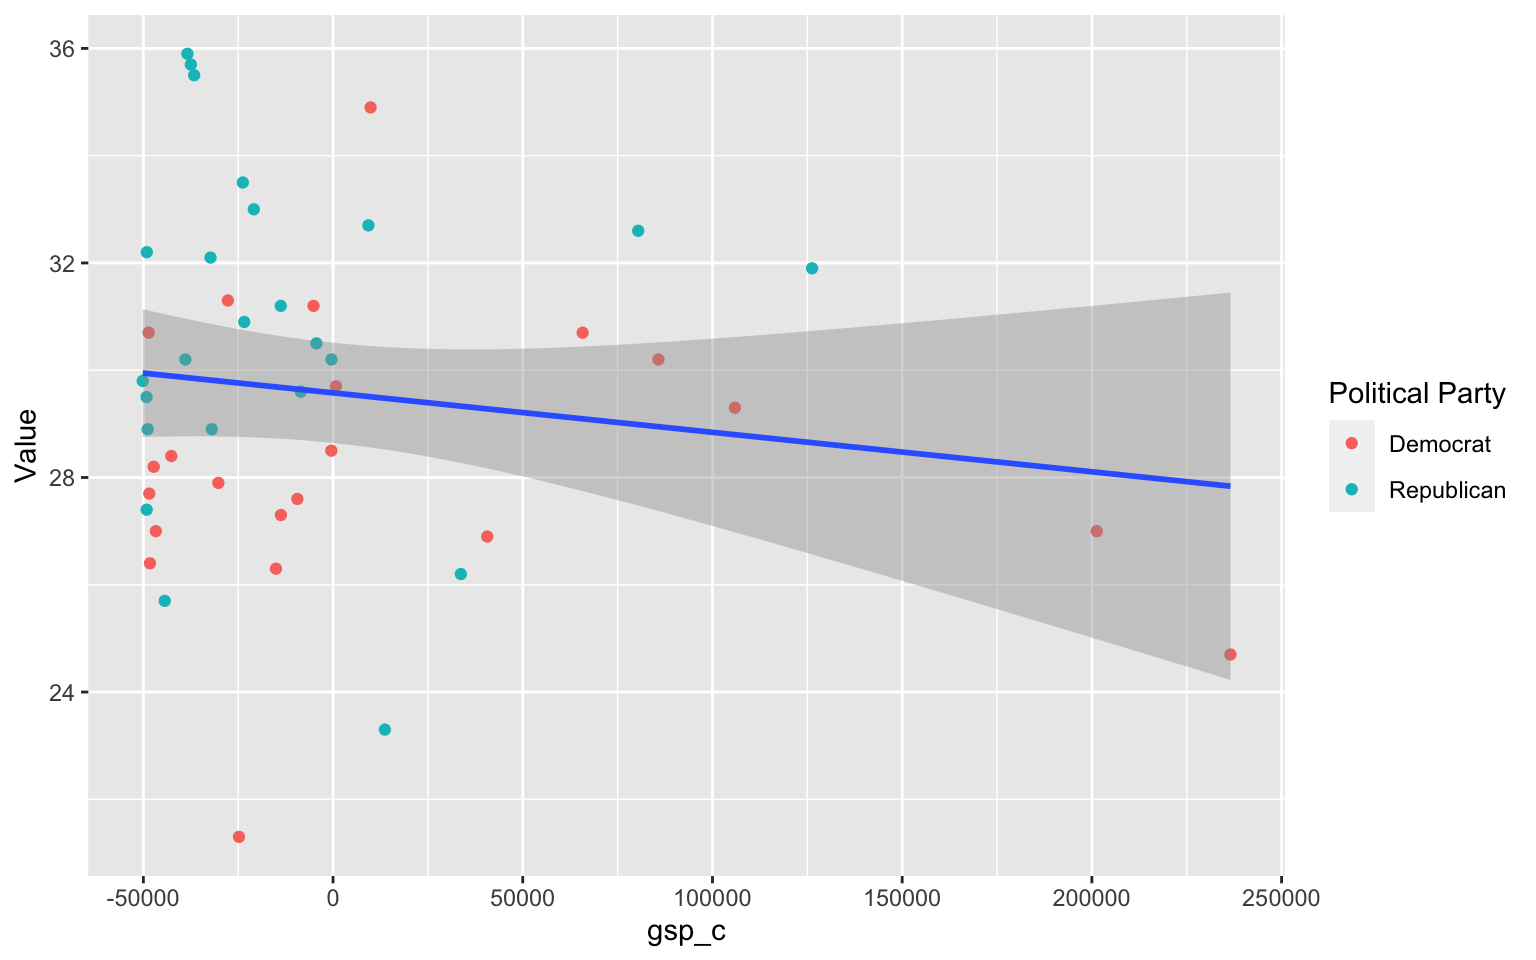
\includegraphics{project1_files/figure-latex/unnamed-chunk-4-1.pdf}

\begin{Shaded}
\begin{Highlighting}[]
\KeywordTok{ggplot}\NormalTok{(}\DataTypeTok{data =}\NormalTok{ merged, }\KeywordTok{aes}\NormalTok{(}\DataTypeTok{x =}\NormalTok{ Murder, }\DataTypeTok{y =}\NormalTok{ Assault, }\DataTypeTok{color =} \StringTok{`}\DataTypeTok{Political Party}\StringTok{`}\NormalTok{)) }\OperatorTok{+}
\StringTok{  }\KeywordTok{geom_point}\NormalTok{(}\DataTypeTok{size =} \DecValTok{3}\NormalTok{) }\OperatorTok{+}\StringTok{ }\KeywordTok{ggtitle}\NormalTok{(}\StringTok{"Scatterplot of Murder vs Assault between Democratic and Republican States"}\NormalTok{)}
\end{Highlighting}
\end{Shaded}

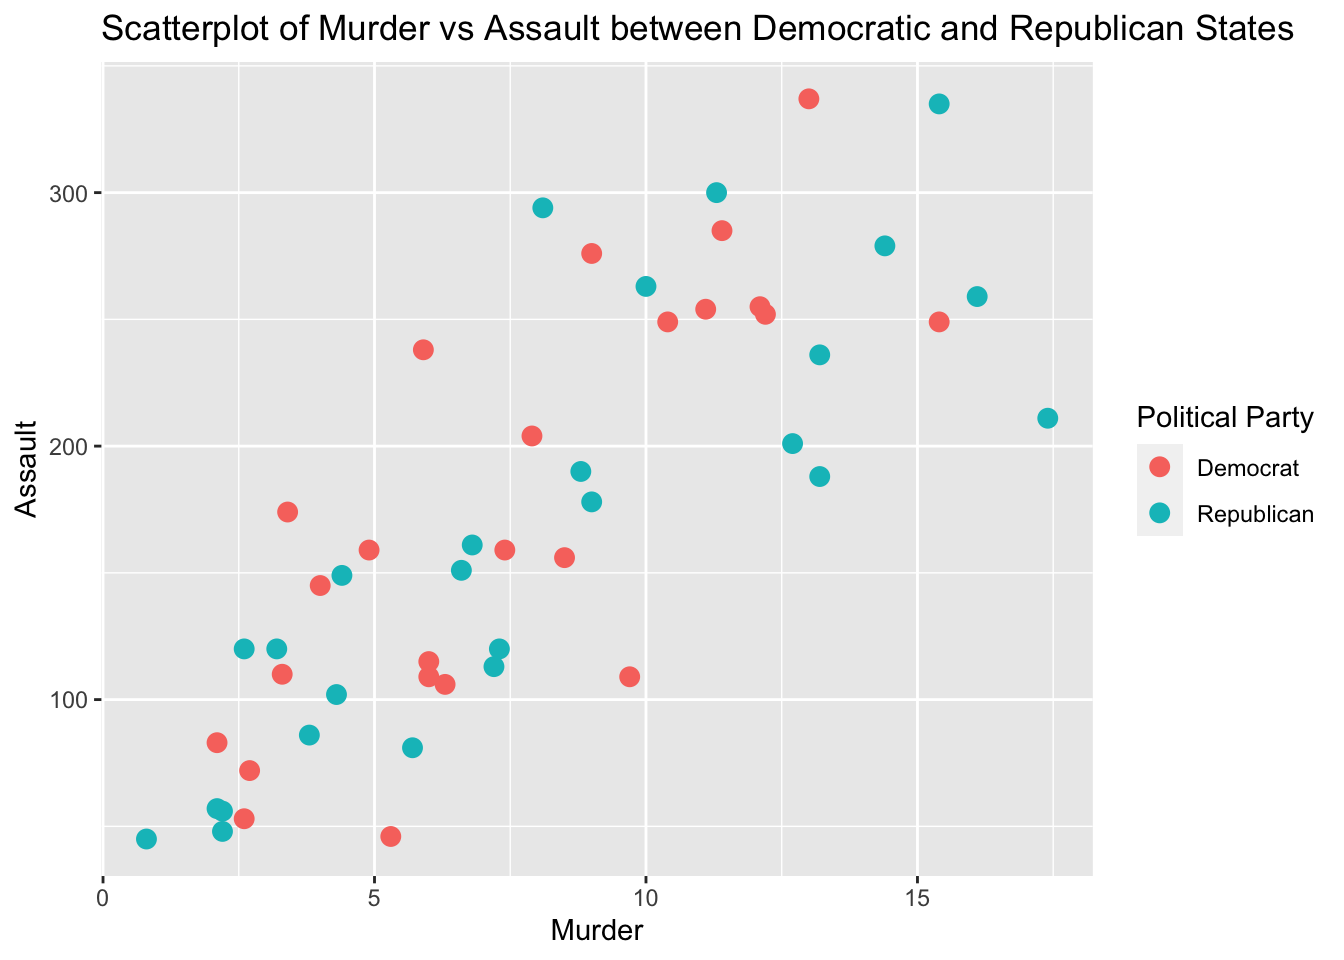
\includegraphics{project1_files/figure-latex/unnamed-chunk-4-2.pdf}

\begin{Shaded}
\begin{Highlighting}[]
\KeywordTok{ggplot}\NormalTok{(merged_total, }\KeywordTok{aes}\NormalTok{(}\DataTypeTok{x=}\StringTok{`}\DataTypeTok{Poverty Percent, All Ages}\StringTok{`}\NormalTok{, }\DataTypeTok{fill=}\StringTok{`}\DataTypeTok{Political Party}\StringTok{`}\NormalTok{)) }\OperatorTok{+}\StringTok{ }\KeywordTok{scale_fill_brewer}\NormalTok{(}\DataTypeTok{palette =} \StringTok{"Pastel1"}\NormalTok{)}\OperatorTok{+}\StringTok{  }\KeywordTok{theme}\NormalTok{(}\DataTypeTok{legend.position=}\KeywordTok{c}\NormalTok{(.}\DecValTok{9}\NormalTok{,.}\DecValTok{7}\NormalTok{)) }\OperatorTok{+}\StringTok{ }\KeywordTok{geom_density}\NormalTok{(}\DataTypeTok{alpha=}\NormalTok{.}\DecValTok{75}\NormalTok{) }\OperatorTok{+}\KeywordTok{ggtitle}\NormalTok{(}\StringTok{"Density Graph of Poverty Percent Between Democrat & Republican States"}\NormalTok{)}
\end{Highlighting}
\end{Shaded}

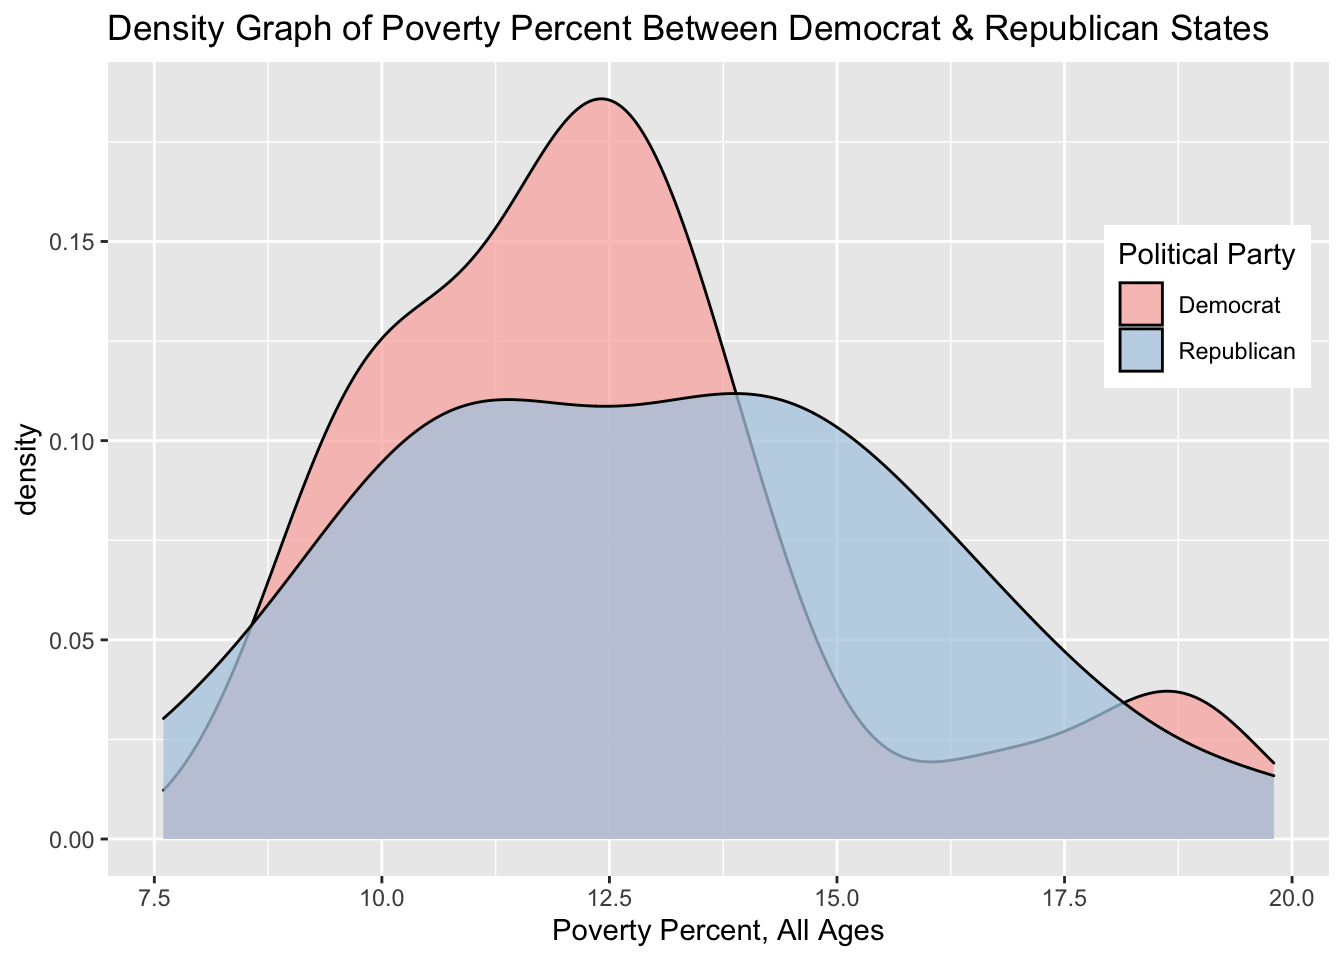
\includegraphics{project1_files/figure-latex/unnamed-chunk-4-3.pdf}

\begin{Shaded}
\begin{Highlighting}[]
\KeywordTok{ggplot}\NormalTok{(merged_total, }\KeywordTok{aes}\NormalTok{(}\DataTypeTok{x =} \StringTok{`}\DataTypeTok{Political Party}\StringTok{`}\NormalTok{, }\DataTypeTok{y =}\NormalTok{ average_arrest, }\DataTypeTok{fill=}\StringTok{`}\DataTypeTok{Political Party}\StringTok{`}\NormalTok{))}\OperatorTok{+}
\KeywordTok{geom_bar}\NormalTok{(}\DataTypeTok{stat=}\StringTok{"summary"}\NormalTok{,}\DataTypeTok{fun.y=}\StringTok{"mean"}\NormalTok{)}\OperatorTok{+}\StringTok{ }\KeywordTok{scale_fill_brewer}\NormalTok{(}\DataTypeTok{palette =} \StringTok{"Pastel1"}\NormalTok{)}\OperatorTok{+}
\KeywordTok{geom_errorbar}\NormalTok{(}\DataTypeTok{stat=}\StringTok{"summary"}\NormalTok{, }\DataTypeTok{width=}\NormalTok{.}\DecValTok{5}\NormalTok{) }\OperatorTok{+}\StringTok{ }\KeywordTok{theme}\NormalTok{(}\DataTypeTok{legend.position =} \StringTok{"none"}\NormalTok{) }\OperatorTok{+}\StringTok{ }\KeywordTok{ggtitle}\NormalTok{(}\StringTok{"Average Arrests for Democrat vs Republican States"}\NormalTok{)}
\end{Highlighting}
\end{Shaded}

\begin{verbatim}
## Warning: Ignoring unknown parameters: fun.y
\end{verbatim}

\begin{verbatim}
## No summary function supplied, defaulting to `mean_se()`
## No summary function supplied, defaulting to `mean_se()`
\end{verbatim}

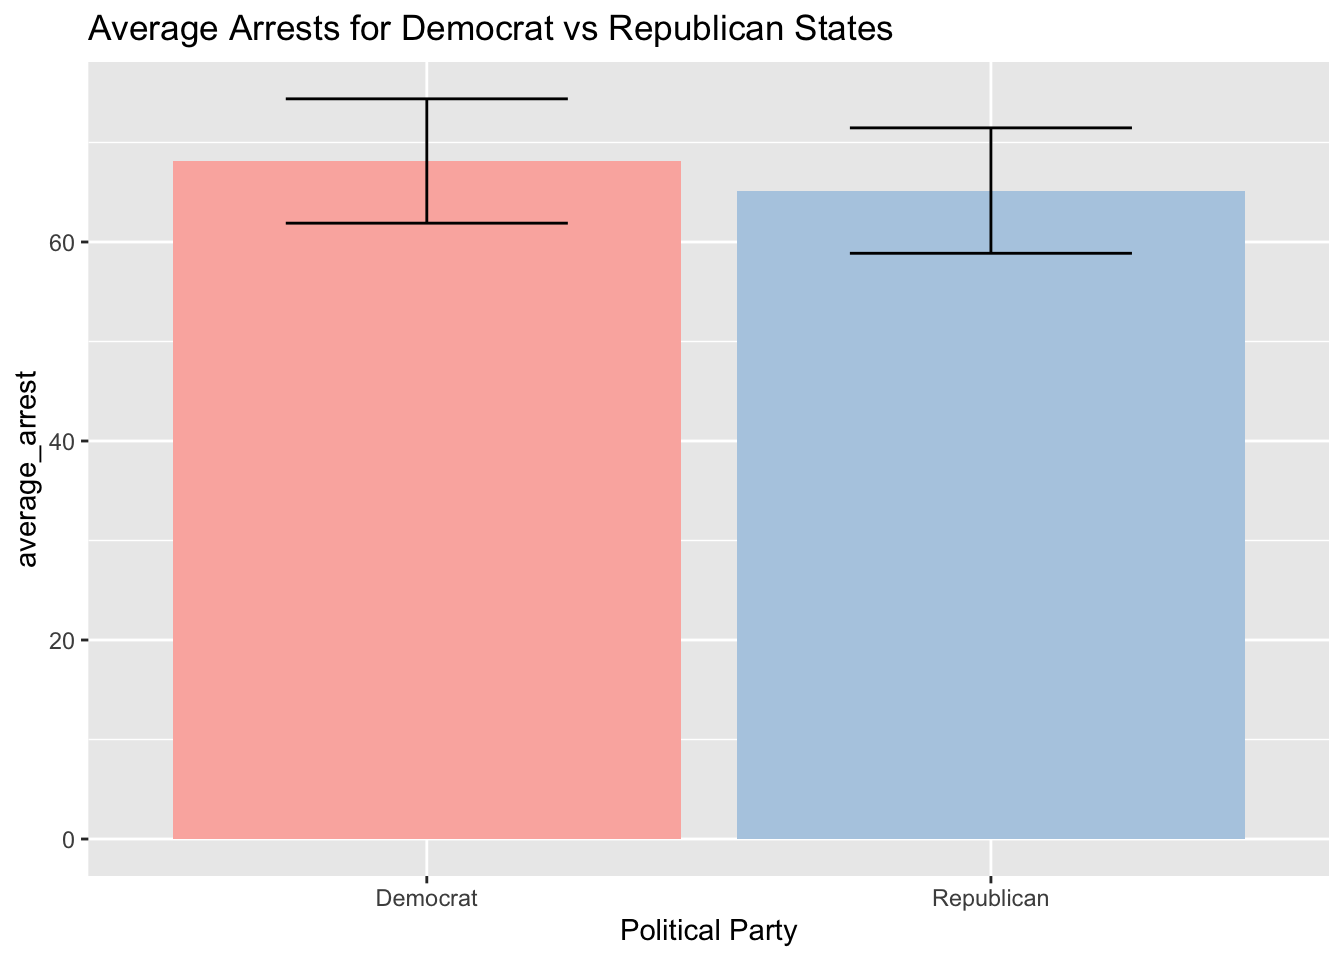
\includegraphics{project1_files/figure-latex/unnamed-chunk-4-4.pdf}

I created a correlation heat map, density graph, scatterplot, and a bar
graph. The correlation heat map displayed the correlation between the
numeric variables. The correlation values were color-coded in order to
help visualize and easily depict the correlation value between the
numeric values. The correlation heatmap showed that Murder and Assault
had the highest correlation of .8, Rape and Assault had a moderate
correlation of .67, and the lowest correlation of .13 between Poverty
Percentage and Rape. For the scatterplot, both democrat and republican
states showed a best fit linear correlation for muder and assault
relationship. This tells us that no matter what political party the
state identifies as, the more murder there appears to be, the more
assault there appears to be. This can be further supported by the
correlation of .8 from the correlation heat map. The density graph shows
the poverty percent of each state and its political party. It easily
depicts the skewness of the graphs. The density graphs shows us that
Republican states have a general spread across poverty percent where
Democratic states are higher around 10-12.5, and decreases around 15+.
The bar graph shows that democratic states have generally higher arrests
but because the standard error bars overlap, we cannot say this is
significant information.

\textbf{Dimensionality Reduction}

\begin{Shaded}
\begin{Highlighting}[]
\CommentTok{#Dimensionality Reduction}
\KeywordTok{library}\NormalTok{(cluster)}
\NormalTok{pam_dat<-merged_total}\OperatorTok\KeywordTok{select}\NormalTok{(Rape, Murder, Assault, }\StringTok{`}\DataTypeTok{Poverty Percent, All Ages}\StringTok{`}\NormalTok{)}
\NormalTok{sil_width<-}\KeywordTok{vector}\NormalTok{()}
\ControlFlowTok{for}\NormalTok{(i }\ControlFlowTok{in} \DecValTok{2}\OperatorTok{:}\DecValTok{10}\NormalTok{)\{}
\NormalTok{pam_fit <-}\StringTok{ }\KeywordTok{pam}\NormalTok{(pam_dat, }\DataTypeTok{diss =} \OtherTok{TRUE}\NormalTok{, }\DataTypeTok{k =}\NormalTok{ i)}
\NormalTok{sil_width[i] <-}\StringTok{ }\NormalTok{pam_fit}\OperatorTok{$}\NormalTok{silinfo}\OperatorTok{$}\NormalTok{avg.width}
\NormalTok{\}}
\end{Highlighting}
\end{Shaded}

\begin{verbatim}
## Warning in as.dist.default(x): non-square matrix

## Warning in as.dist.default(x): non-square matrix

## Warning in as.dist.default(x): non-square matrix

## Warning in as.dist.default(x): non-square matrix

## Warning in as.dist.default(x): non-square matrix

## Warning in as.dist.default(x): non-square matrix

## Warning in as.dist.default(x): non-square matrix

## Warning in as.dist.default(x): non-square matrix

## Warning in as.dist.default(x): non-square matrix
\end{verbatim}

\begin{Shaded}
\begin{Highlighting}[]
\KeywordTok{ggplot}\NormalTok{()}\OperatorTok{+}\KeywordTok{geom_line}\NormalTok{(}\KeywordTok{aes}\NormalTok{(}\DataTypeTok{x=}\DecValTok{1}\OperatorTok{:}\DecValTok{10}\NormalTok{,}\DataTypeTok{y=}\NormalTok{sil_width))}\OperatorTok{+}\KeywordTok{scale_x_continuous}\NormalTok{(}\DataTypeTok{name=}\StringTok{"k"}\NormalTok{,}\DataTypeTok{breaks=}\DecValTok{1}\OperatorTok{:}\DecValTok{10}\NormalTok{)}
\end{Highlighting}
\end{Shaded}

\begin{verbatim}
## Warning: Removed 1 row(s) containing missing values (geom_path).
\end{verbatim}

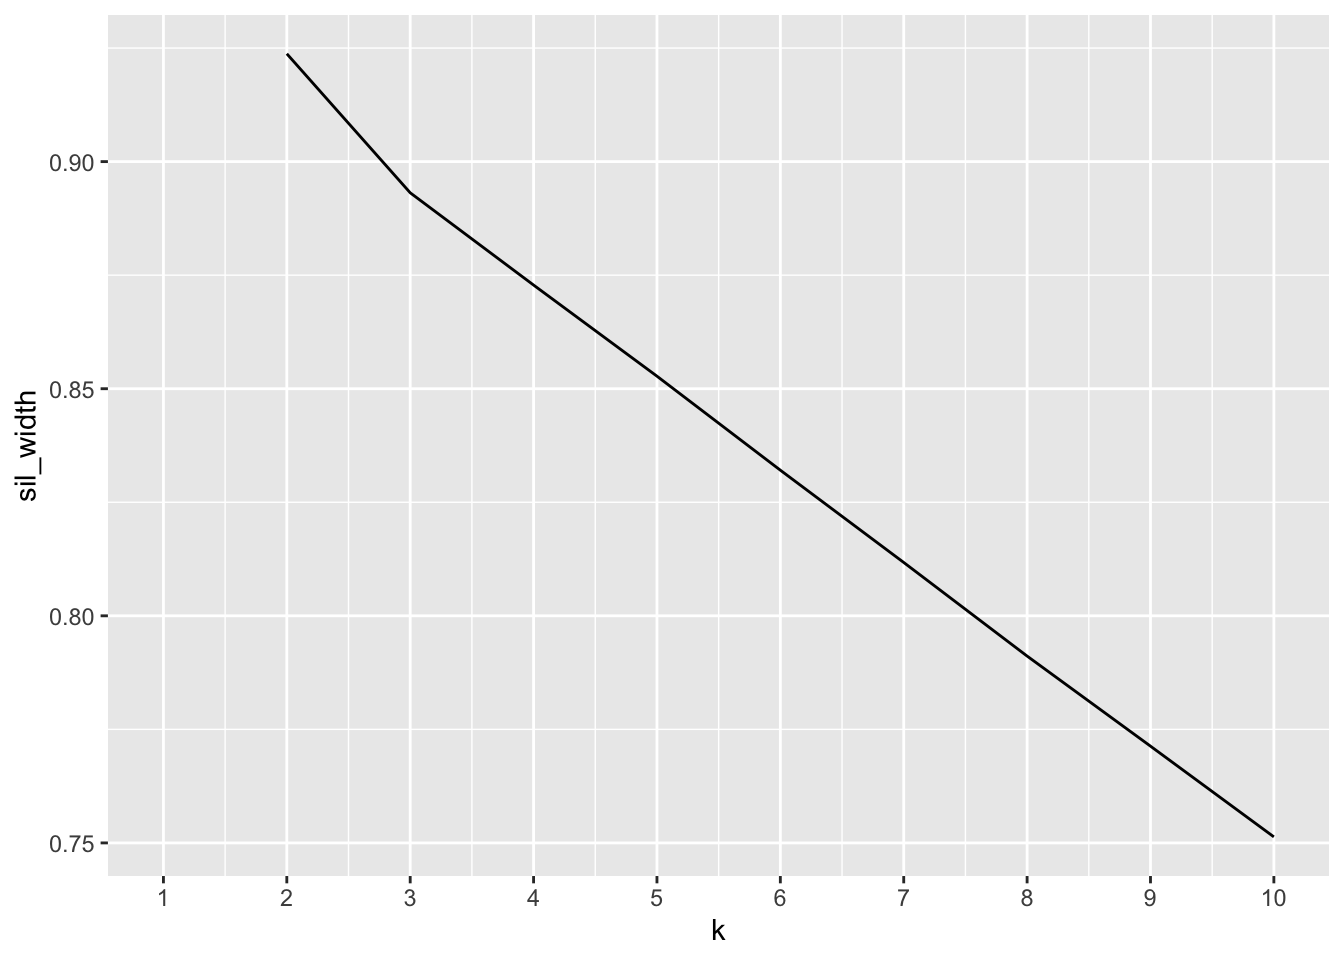
\includegraphics{project1_files/figure-latex/unnamed-chunk-5-1.pdf}

\begin{Shaded}
\begin{Highlighting}[]
\NormalTok{pam1<-pam_dat}\OperatorTok\KeywordTok{pam}\NormalTok{(}\DataTypeTok{k=}\DecValTok{2}\NormalTok{)}
\NormalTok{pam1}
\end{Highlighting}
\end{Shaded}

\begin{verbatim}
## Medoids:
##      ID Rape Murder Assault Poverty Percent, All Ages
## [1,] 32 26.1   11.1     254                      13.7
## [2,] 26 16.4    6.0     109                      12.9
## Clustering vector:
##  [1] 1 1 1 1 1 1 2 1 1 1 2 2 1 2 2 2 2 1 2 1 2 1 2 1 2 2 2 1 2 2 1 1 1 2 2 2 2 2
## [39] 2 1 2 1 1 2 2 2 2 2 2 2
## Objective function:
##    build     swap 
## 42.76792 34.60428 
## 
## Available components:
##  [1] "medoids"    "id.med"     "clustering" "objective"  "isolation" 
##  [6] "clusinfo"   "silinfo"    "diss"       "call"       "data"
\end{verbatim}

\begin{Shaded}
\begin{Highlighting}[]
\NormalTok{pamclust<-pam_dat }\OperatorTok\StringTok{ }\KeywordTok{mutate}\NormalTok{(}\DataTypeTok{cluster=}\KeywordTok{as.factor}\NormalTok{(pam1}\OperatorTok{$}\NormalTok{clustering))}
\NormalTok{pamclust }\OperatorTok\StringTok{ }\KeywordTok{ggplot}\NormalTok{(}\KeywordTok{aes}\NormalTok{(Murder,Assault,}\DataTypeTok{color=}\NormalTok{cluster)) }\OperatorTok{+}\StringTok{ }\KeywordTok{geom_point}\NormalTok{()}
\end{Highlighting}
\end{Shaded}

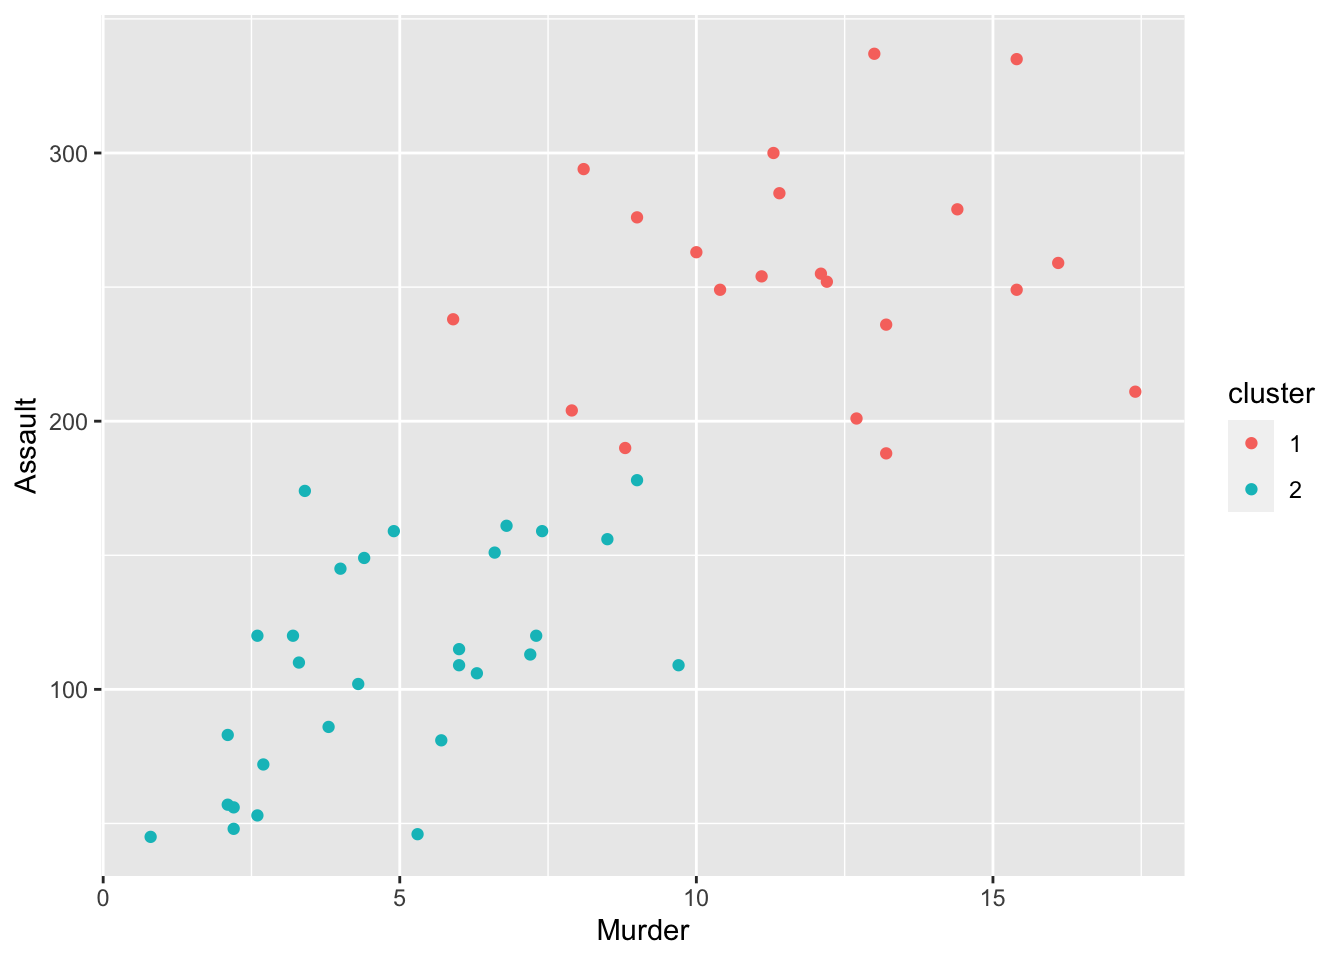
\includegraphics{project1_files/figure-latex/unnamed-chunk-5-2.pdf}

\begin{Shaded}
\begin{Highlighting}[]
\NormalTok{pamclust }\OperatorTok\StringTok{ }\KeywordTok{group_by}\NormalTok{(cluster) }\OperatorTok\StringTok{ }\KeywordTok{summarize_if}\NormalTok{(is.numeric,mean,}\DataTypeTok{na.rm=}\NormalTok{T)}
\end{Highlighting}
\end{Shaded}

\begin{verbatim}
## # A tibble: 2 x 5
##   cluster  Rape Murder Assault `Poverty Percent, All Ages`
##   <fct>   <dbl>  <dbl>   <dbl>                       <dbl>
## 1 1        28.1  11.9     255                         14.3
## 2 2        16.2   4.84    110.                        11.7
\end{verbatim}

\begin{Shaded}
\begin{Highlighting}[]
\NormalTok{pam1}\OperatorTok{$}\NormalTok{silinfo}\OperatorTok{$}\NormalTok{avg.width}
\end{Highlighting}
\end{Shaded}

\begin{verbatim}
## [1] 0.6198666
\end{verbatim}

\begin{Shaded}
\begin{Highlighting}[]
\KeywordTok{library}\NormalTok{(GGally)}
\end{Highlighting}
\end{Shaded}

\begin{verbatim}
## Registered S3 method overwritten by 'GGally':
##   method from   
##   +.gg   ggplot2
\end{verbatim}

\begin{verbatim}
## 
## Attaching package: 'GGally'
\end{verbatim}

\begin{verbatim}
## The following object is masked from 'package:dplyr':
## 
##     nasa
\end{verbatim}

\begin{Shaded}
\begin{Highlighting}[]
\NormalTok{pamclust}\OperatorTok\KeywordTok{ggpairs}\NormalTok{(}\DataTypeTok{columns=}\DecValTok{1}\OperatorTok{:}\DecValTok{4}\NormalTok{,}\KeywordTok{aes}\NormalTok{(}\DataTypeTok{color=}\NormalTok{cluster))}
\end{Highlighting}
\end{Shaded}

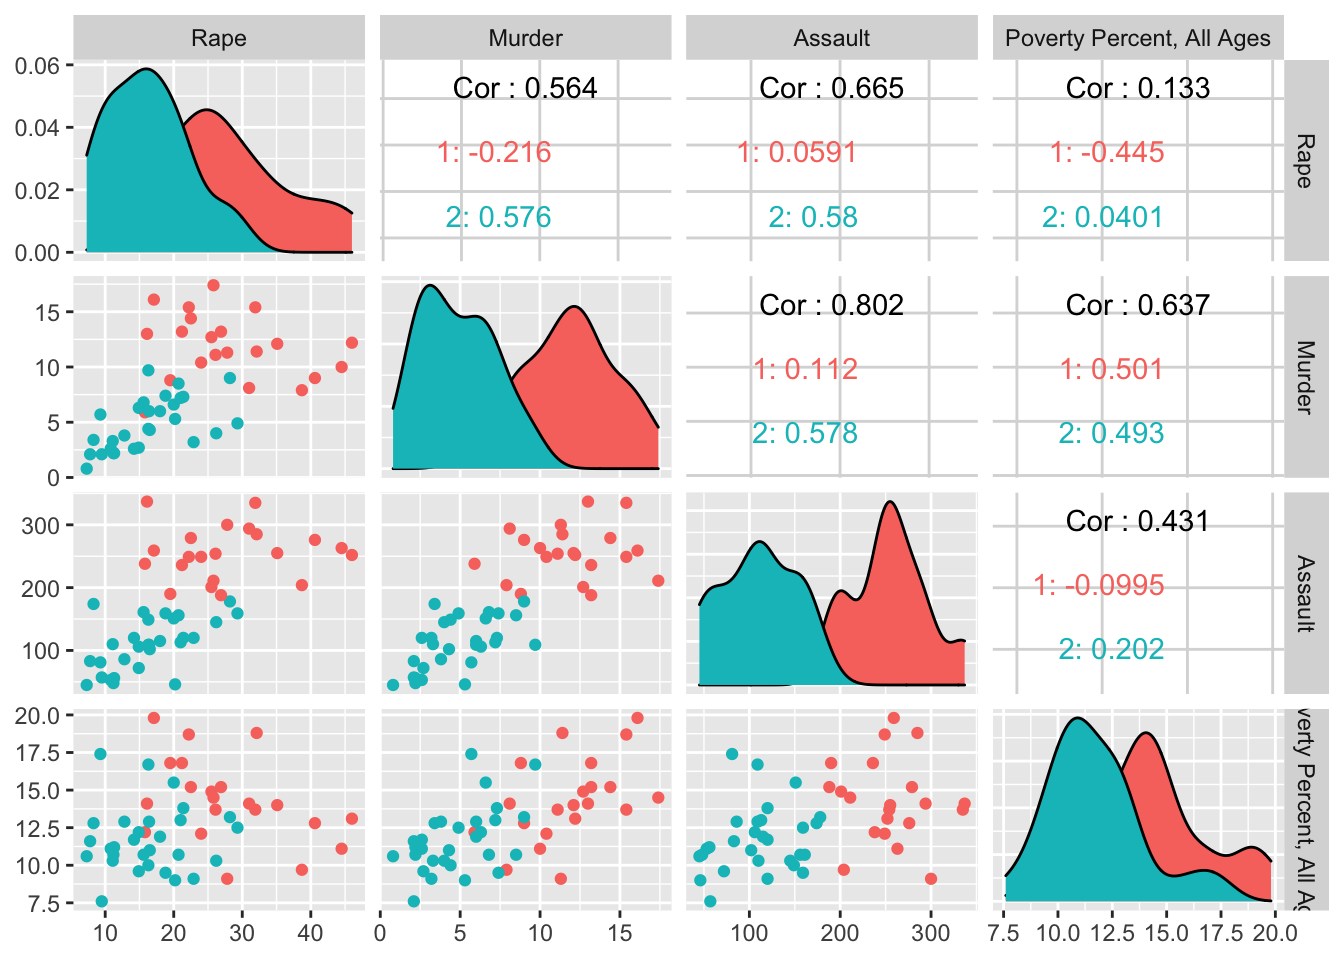
\includegraphics{project1_files/figure-latex/unnamed-chunk-5-3.pdf}

I found out the best k to use was 2. Setting my k equal to 2, I
performed PAM clustering and 2 clusters were found distinctly (you could
even say there is a good vs a bad cluster - low vs high cluster in
crime). Furthermore, the ggpairs shows us the different clusters that
could have been made and how the original cluster of murder and assault
we made was the best cluster graph.

\end{document}
